\documentclass[a4paper,11pt,oneside]{article}

\usepackage[utf8]{inputenc}
\usepackage[T1]{fontenc}
\usepackage[ngerman]{babel}
\usepackage{amssymb}
\usepackage{amsmath}
\usepackage{graphicx}
\usepackage{float}
\usepackage{hyperref}
\usepackage[dvipsnames]{xcolor}
\usepackage{listings}
\usepackage[top=2cm, bottom=2.5cm, right=2.5cm, left=2.5cm]{geometry}

\renewcommand{\familydefault}{\sfdefault}
\parindent0pt
\parskip6pt
\hypersetup{colorlinks=true,urlcolor=blue,linkcolor=blue}
\lstset{basicstyle=\ttfamily\small, mathescape, literate={Ö}{{\"O}}1 {Ä}{{\"A}}1 {Ü}{{\"U}}1 {ß}{{\ss}}1 {ü}{{\"u}}1 {ä}{{\"a}}1 {ö}{{\"o}}1}

\begin{document}

\title{Kurzzusammenfassung:\\Methoden der statistischen Qualitätssicherung}
\author{Alexander Herzog\\\href{mailto:alexander.herzog@tu-clausthal.de}{\small\texttt{alexander.herzog@tu-clausthal.de}}}
\date{}

\maketitle

Methoden der statistischen Qualitätssicherung kommen sowohl zur Überwachung laufender Prozesse als auch bei der Prüfung von Wareneingängen zum Einsatz. Während das Ziel bei der Prozessüberwachung darin besteht, kontinuierlich zu prüfen, dass sich die Parameter eines (Fertigungs-)Prozesses innerhalb der jeweiligen Soll-Bereiche befinden, geht es bei der statistischen Überwachung von Wareneingängen darum, die Qualität angelieferter Werkstücke sicherzustellen, ohne dabei eine \emph{Vollkontrolle} durchführen zu müssen. Häufig sind Vollkontrollen entweder nicht möglich, da das zu prüfende Werkstück bei der Prüfung zerstört wird, oder aber eine Vollkontrolle wäre wirtschaftlich nicht sinnvoll:

\begin{itemize}
\item
Chargen von angelieferte Silvesterraketen können nicht vor dem Verkauf einer Vollkontrolle unterzogen werden.
\item
Bei großen Lieferungen von Schrauben, Unterlegscheiben und ähnlichen Kleinteilen in einer Fertigung wäre ein Vollkontrolle zwar möglich, aber mit Blick auf den Wert der einzelnen Bauteile nicht wirtschaftlich.
\end{itemize}



\section{Stichprobenprüfung}

Statt einer Vollkontrolle wird daher in diesen Fällen nur eine Stichprobe (der Größe $n\in\mathbb N$) der Lieferung (der Größe $N\in\mathbb N$ mit $N$ deutlich größer als $n$) geprüft. Voraussetzung für die folgenden Überlegungen ist, dass eine \emph{Gut-Schlecht-Prüfung} möglich ist, d.\,h.\ dass bei einem Werkstück eindeutig bestimmt werden kann, ob dieses die definierten Anforderungen erfüllt oder nicht. Es handelt sich also um eine Ja/Nein-Unterscheidung. Bei einer Vollkontrolle würden Lieferant und Kunde eine eindeutige Qualitätsgrenze für Lieferungen festlegen -- z.\,B.\ $p=0{,}1\,\%$. Sind von $N=10.000$ gelieferten Schrauben höchstens $N\cdot p=10.000\cdot0{,}1\%=10$ fehlerhaft, so wird die Lieferung angenommen. Andernfalls wird sie an den Lieferanten zurückgeschickt. Bei einer Stichprobenprüfung sind solche absoluten Aussagen nicht mehr möglich.



\section{Gut- und Schlechtgrenze}

Daher einigen sich Lieferant und Kunde auf eine \emph{Gutgrenze} (Acceptance Quality Limit, AQL) und eine \emph{Schlechtgrenze} (Limiting Quality; LQ). Lieferungen, die die Gutgrenze einhalten, sollen ,,fast immer'' angenommen werden. Lieferungen, die in Bezug auf den Anteil an Ausschussteilen die Schlechtgrenze verletzen, sollen ,,fast nie'' angenommen werden. Schiebt man Gut- und Schlechtgrenze immer näher zusammen, so nähert sich der Stichprobenplan immer mehr einer Vollkontrolle.

\subsection*{Bezeichnungen für Gut- und Schlechtgrenze}

\begin{eqnarray*}
p_{1-\alpha}&:=&\text{Gutgrenze; Ausschussanteil bei dem Lieferungen fast immer}\\
~&~&\text{angenommen werden sollen}\\[2ex]
1-\alpha&:=&\text{Geforderte minimale Annahmewahrscheinlichkeit für Lieferungen mit einem}\\
~&~&\text{Ausschussanteil von höchstens}~ p_{1-\alpha}\\[2ex]
p_\beta&:=&\text{Schlechtgrenze; Ausschussanteil bei dem Lieferungen fast immer}\\
~&~&\text{abgelehnt werden sollen}\\[2ex]
\beta&:=&\text{Geforderte maximale Annahmewahrscheinlichkeit für Lieferungen mit einem}\\
~&~&\text{Ausschussanteil von}~ p_{\beta} ~\text{oder mehr}
\end{eqnarray*}

\begin{figure}[H]
\begin{center}
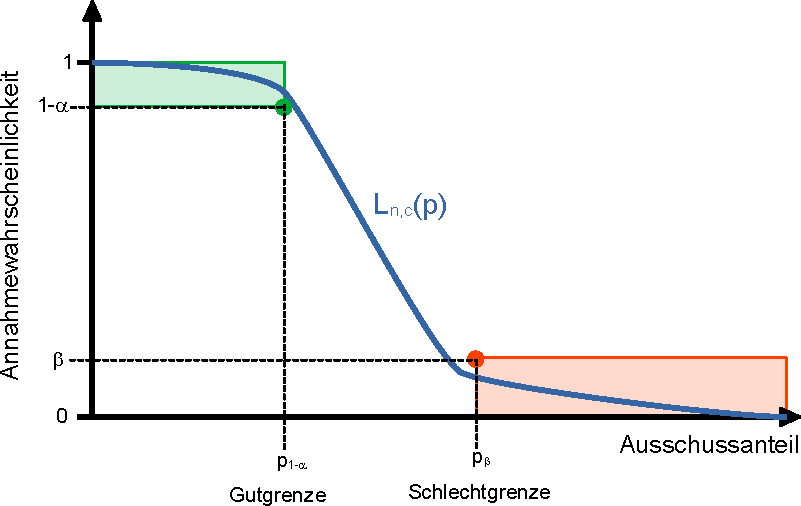
\includegraphics[width=0.7\textwidth]{Operationscharakteristik.pdf}
\end{center}
\caption{Annahmewahrscheinlichkeit, Gut- und Schlechtgrenze bei einer Stichprobenprüfung}
\label{fig:L}
\end{figure}



\section{Fehler 1.\ und 2.\ Art}

Ziel der Festlegung von Gut- und Schlechtgrenze und den zugehörigen Annahmewahrscheinlichkeiten an diesen beiden Qualitätspunkten ist es, ,,gute'' Lieferungen möglichst immer anzunehmen und ,,schlechte'' Lieferungen möglichst immer abzulehnen.

Sagt der Stichprobentest aus, dass die Lieferung gut ist und ist sie dies tatsächlich, oder sagt der Stichprobentest aus, dass die Lieferung schlecht ist und sie ist tatsächlich schlecht, so hat der Test funktioniert. Falls das Stichprobentestergebnis und die Realität bezogen auf die gesamte Lieferung nicht übereinstimmen, hat der Test einen Fehler gemacht:

\begin{itemize}
\item
Wird eine Lieferung auf Basis eines nicht gut ausgefallenen Stichprobentests abgelehnt, obwohl sie in Bezug auf ihre Grundgesamtheit die Qualitätsziele eingehalten hätte, so spricht man von einem \emph{Fehler 1.\ Art} (Lieferantenrisiko).
\item
Wird eine Lieferung auf Basis eines guten Stichprobenergebnissen angenommen, obwohl sie die Qualitätsziele in Bezug auf ihre Grundgesamtheit nicht einhält, so spricht man von einem \emph{Fehler 2.\ Art} (Kundenrisiko).
\end{itemize}

Der Lieferant mögliche gerne den Fehler 1.\ Art minimieren (seine Lieferung wird abgelehnt, obwohl sie gut ist). Der Kunde möchte gern den Fehler 2.\ Art (Lieferung wird angenommen, obwohl sie schlecht ist) minimieren. Über die Wahl von $p_{1-\alpha}$, $1-\alpha$, $p_\beta$ und $\beta$ lassen sich die Wahrscheinlichkeiten für diese Fehler kontrollieren. Je kleiner die Fehlerwahrscheinlichkeiten, die der Stichprobentest liefert, ausfallen sollen, desto mehr gelieferte Werkstücke müssen jeweils kontrolliert werden, d.\,h.\ desto mehr muss sich der Stichprobentest einer Vollkontrolle nähern.

Bei der Festlegung der Gut- und der Schlechtgrenze muss daher immer zwischen der geforderten Qualität an den Test und dem Prüfaufwand abgewogen werden.



\section[n-c-Stichprobenpläne]{$n$-$c$-Stichprobenpläne}

Auf Basis dieser Vorüberlegungen ergibt sich folgendes generelles Vorgehen zur Aufstellung und Anwendung eines Stichprobenplans:

\begin{enumerate}
\item
Lieferant und Kunde einigen sich gemeinsam auf zu erfüllende Qualitätskriterien. Dies kann z.\,B.\ die gemeinsame Festlegung von Gutgrenze ($p_{1-\alpha}$ und $1-\alpha$) und Schlechtgrenze ($p_\beta$ und $\beta$) sein.
\item
Es wird ein Algorithmus angewandt, auf dessen Basis sich ein Stichprobenplan berechnen lässt, der sicherstellt, dass die geforderten Kriterien eingehalten werden. Solch ein Plan schreibt dann vor, dass von Lieferungen der Größe $N\in\mathbb N$ Teilen jeweils $n\in\mathbb N$ Teile geprüft werden müssen. Sind unter diesen $n$ Teilen mehr als $c\in\mathbb N_0$ defekte Teile, so wird die Lieferung zurückgewiesen (und andernfalls wird sie angenommen).
\item
Eintreffenden Lieferungen wird jeweils eine Stichprobe aus $n$ Teilen entnommen. Diese werden geprüft. Sind mehr als $c$ defekte Teile in der Stichprobe enthalten, so wird die Lieferung entweder direkt zurückgewiesen oder aber es wird (wenn dies sinnvoll möglich ist) eine Vollkontrolle durchgeführt.
\end{enumerate}



\section{Operationscharakteristik}

Bei der Entnahme und Prüfung einer Stichprobe aus einer Grundgesamtheit handelt es sich aus Sicht der Stochastik um ein \emph{Urnenmodell}:

\begin{itemize}
\item
In einer Urne sind $N\in\mathbb N$ Kugeln enthalten (Gesamtgröße der Lieferung).
\item
Der Urne werden $n\in\mathbb N$ Kugeln ohne Zurücklegen entnommen, wobei $n\le N$ ist (Stichprobengröße).
\item
Die Anzahl an roten Kugeln (defekte Werkstücke) betrage $R\in\mathbb N_0$, wobei offensichtlich $R\le N$ ist. Im Falle einer Lieferung ist $R$ unbekannt.
\item
Aus $R$ (unbekannt) und $N$ (bekannt) lässt sich dann auch der Anteil der roten Kugeln bzw.\ defekten Bauteile bestimmen: $p=\frac{R}{N}$.
\end{itemize}

Urnenmodelle im Falle des Ziehens ohne Zurücklegen werden durch die \emph{Hypergeometrische Verteilung} beschrieben. Gemäß dieser beträgt die Wahrscheinlichkeit genau $k\in\mathbb N_0$, $k=0,\ldots,n$, rote Kugeln bzw.\ defekte Bauteile zu ziehen bzw.\ in der Stichprobe zu haben:
$$
P(X=k)=
\mathrm{Hg}_{N,R,n}(k)=
\frac{\binom{R}{k}\binom{N-R}{n-k}}{\binom{N}{n}}.
$$
Die Wahrscheinlichkeit, dass eine Stichprobe der Größe $n$ aus einer Lieferung aus $N$ Teilen (und darunter $R$ defekten Teilen) höchstens $c\in\mathbb N_0$ defekte Teile enthält, beträgt damit:
$$
P(X\le c)=
\sum_{k=0}^c \mathrm{Hg}_{N,R,n}(k)=
\sum_{k=0}^c \frac{\binom{R}{k}\binom{N-R}{n-k}}{\binom{N}{n}}.
$$
Mit der Näherung $p\approx\frac{R}{N}$ bzw.\ $R:=\lfloor N\cdot p\rfloor$ nennt man
$$
L_{n,c}(p):=
P(X\le c)=
\sum_{k=0}^c \frac{\binom{\lfloor N\cdot p\rfloor}{k}\binom{N-\lfloor N\cdot p\rfloor}{n-k}}{\binom{N}{n}}
$$
die \emph{Operationscharakteristik} des $n$-$c$-Stichprobenplans (siehe auch Abbildung \ref{fig:L}).



\section[Konstruktion von n-c-Stichprobenplänen]{Konstruktion von $n$-$c$-Stichprobenplänen}

Ziel ist es jetzt, eine Operationscharakteristik $L_{n,c}(p)$ (bzw.\ genauer Parameter $n$ und $c$) zu finden, so dass

\begin{enumerate}
\item
die Operationscharakteristik die Bedingung an der Gutgrenze erfüllt:\\
$L_{n,c}(p_{1-\alpha})\ge1-\alpha$,
\item
die Bedingung an der Schlechtgrenze erfüllt: $L_{n,c}(p_\beta)\le\beta$ und
\item
der Prüfaufwand minimal ist: $n\to\mathrm{Min}$.
\end{enumerate}

\subsection{Algorithmus von Günther}

Generell gilt, dass die Annahme einer Lieferung immer unwahrscheinlicher wird, je mehr Teile $n$ geprüft werden (bei einer festen maximal zulässigen Anzahl an fehlerhaften Teilen $c$ in der Stichprobe). Gleichzeitig gilt, dass die Annahme einer Lieferung um so wahrscheinlicher wird, je mehr defekte Teile $c$ (bei einer konstanten Stichprobengröße $n$) zugelassen werden. Daraus folgt:

\begin{itemize}
\item
Erfüllt die Operationscharakteristik die Gutgrenze nicht (gute Lieferungen werden mit einer zu hohen Wahrscheinlichkeit abgewiesen), erhöht man $c$ (und verschiebt die Operationscharakteristik damit nach oben).
\item
Erfüllt die Operationscharakteristik die Schlechtgrenze nicht (schlechte Lieferungen werden mit einer zu hohen Wahrscheinlichkeit angenommen), erhöht man $n$ (und verschiebt die Operationscharakteristik damit nach unten).
\end{itemize}

Systematisch zusammenfasst wird diese Vorgehensweise im Algorithmus von Günther:

\begin{enumerate}
\item
\emph{Initialisierung ($n:=1$, $c:=0$):}~\\
Begonnen wird mit einer Stichprobe vom Umfang $n:=1$ in der für eine Annahme der gesamten Lieferung kein defektes Bauteil enthalten sein darf ($c:=0$).
\item
\emph{Prüfen, ob der Plan die Bedingungen erfüllt ({\color{ForestGreen}$L_{n,c}(p_{1-\alpha})\ge1-\alpha$} $\wedge$ {\color{ForestGreen}$L_{n,c}(p_\beta)\le\beta$} ?):}~\\
Erfüllt dieser Stichprobenplan sowohl die Gut- als auch die Schlechtgrenze, so ist das Verfahren beendet und ein optimaler Stichprobenplan (d.\,h.\ ein Stichprobenplan mit minimaler Stichprobengröße) ist gefunden.
\item
\emph{{\color{Red}$L_{n,c}(p_\beta)>\beta$} $\to$ $n:=n+1$:}~\\
Erfüllt der Stichprobenplan die Schlechtgrenze noch nicht (schlechte Lieferungen werden mit einer zu hohen Wahrscheinlichkeit angenommen), so wird $n$ erhöht. Danach wird dieser Schritt noch einmal ausgeführt.
\item
\emph{{\color{Red}$L_{n,c}(p_{1-\alpha})<1-\alpha$} $\to$ $c:=c+1$, $n:=c$:}~\\
Erfüllt der Plan (bedingt durch Schritt 3) nun zwar die Schlechtgrenze, aber noch nicht die Gutgrenze, so wird $c$ um eins erhöht, $n$ auf den kleinstmöglich sinnvollen Wert ($c$) gesetzt und mit Schritt 3 fortgesetzt.
\item
\emph{Ende ({\color{ForestGreen}$L_{n,c}(p_{1-\alpha})\ge1-\alpha$} $\wedge$ {\color{ForestGreen}$L_{n,c}(p_\beta)\le\beta$}):}~\\
Bedingt durch die beiden vorherigen Schritte ist sichergestellt, dass der Plan sowohl die Gut- als auch die Schlechtgrenze einhält.
\end{enumerate}

In Pseudocode lässt sich der Algorithmus von Günther wie folgt formulieren:

\begin{lstlisting}[inputencoding={utf8},frame=single]
// Initialisierung
n:=1
c:=0

// Schon fertig?
if ($L_{n,c}(p_{1-\alpha})\ge1-\alpha$ && $L_{n,c}(p_\beta)\le\beta$) $\to$ Ende

// Äußere Schleife: c erhöhen
while (true) {
  // Innere Schleife: n erhöhen bis Schlechtgrenze eingehalten wird
  while ($L_{n,c}(p_\beta)>\beta$) {
    n++
  }
  // Gutgrenze auch erfüllt?
  if ($L_{n,c}(p_{1-\alpha})\ge1-\alpha$) $\to$ Ende

  // Sonst c erhöhen und nächste Runde in äußerer Schleife
  c++
  n:=c
}
\end{lstlisting}

\subsection[Chi-Quadrat-Methode]{$\chi^2$-Methode}

Zur Ermittlung eines optimalen Stichprobenplans auf Basis des Algorithmus von Günther müssen zwei ineinander Verschachtelte Schleifen ausgeführt werden. In jedem Schritt der inneren Schleife muss $L_{n,c}(p)$ berechnet werden, welches wiederum eine Summe über einem Bruch aus drei Binomialkoeffizienten ist. Zur Berechnung eines Binomialkoeffizienten muss ein Produkt über jeweils eine ganze Reihe von Faktoren bestimmt werden. Damit hat der Algorithmus eine Gesamtkomplexität von $O(n^4)$. Wird die Berechnung per Computer ausgeführt, so stellt diese Komplexität kein Problem dar. Bei einer Berechnung mit Stift und Papier wäre der Aufwand jedoch erheblich. Daher wurde als die Notwendigkeit einer Stichprobenprüfung mit dem Aufkommen der industriellen Massenproduktion entstand nach einer (approximativen) Methode mit einer geringeren Komplexität gesucht.

Die $\chi^2$-Methode liefert genau dies: Ist der Lieferumgang $N$ groß und der erwartete Anteil an defekten Bauteilen $p$ klein, so kann statt des Ziehens ohne Zurücklegen (Hypergeometrische Verteilung) zur \emph{Poisson-Verteilung} übergegangen werden:

$$
P(X=k)=\frac{\lambda^k}{k!}\exp(-\lambda),
$$
wobei $\lambda:=n\cdot p$ ist. Weiter ist:

\begin{equation}\label{eq:LPoisson}
P(X\le c)=
\sum_{k=0}^c \frac{\lambda^k}{k!}\exp(-\lambda)=
1-G(2\lambda,2(c+1)),
\end{equation}
wobei $G$ die $\chi^2$-Verteilung mit $2(c+1)$ Freiheitsgraden ist.

Nimmt man also an, dass für die Operationscharakteristik $L_{n,c}(p):=1-G(2np,2(c+1))$ gilt, so lassen sich die Bedingungen für die Gut- und die Schlechtgrenze ($L_{n,c})(p_{1-\alpha})\ge1-\alpha$ und $L_{n,c}(p_\beta)\le\beta$) wie folgt umschreiben:

\begin{align*}
L_{n,c}(p_{1-\alpha}) \ge 1-\alpha
&\iff 1-G(2np_{1-\alpha},2(c+1))\ge1-\alpha\\
&\iff G(2np_{1-\alpha},2(c+1)) \le\alpha\\
&\iff G^{-1}(\alpha,2(c+1))\ge2np_{1-\alpha}\\
&\iff \frac{G^{-1}(\alpha,2(c+1))}{2p_{1-\alpha}}\ge n,\\[2ex]
L_{n,c}(p_\beta)\le\beta
&\iff 1-G(2np_\beta,2(c+1))\le\beta\\
&\iff G(2np_\beta,2(c+1))\ge1-\beta\\
&\iff G^{-1}(1-\beta,2(c+1))\le2np_\beta\\
&\iff \frac{G^{-1}(1-\beta,2(c+1))}{2p_\beta}\le n
\end{align*}

Der Algorithmus zur Bestimmung von $n$ und $c$ lässt sich dann auf eine Iteration über $c$ zurückführen. In jedem Iterationsschritt müssen zwei Werte des Inversen der $\chi^2$-Verteilung berechnet werden. Diese Werte liegen (für die Arbeit mit Stift und Papier) üblicherweise tabelliert vor, so dass hier keine Berechnungen notwendig sind, sondern nur jeweils zwei Werte aus einer Tabelle abgelesen werden müssen. Damit ergibt sich folgende Rechenvorschrift:

Es sei $G(x,k)$ die Verteilungsfunktion der $\chi^2$-Verteilung in $k\in\mathbb N$ Freiheitsgraden an der Stelle $x\ge0$. Dann wird $c$ so lange erhöht, bis folgende Ungleichungen beide erfüllt sind:

$$
\frac{G^{-1}(1-\beta;2(c+1))}{2p_\beta}\le n\le\frac{G^{-1}(\alpha;2(c+1))}{2p_{1-\alpha}}.
$$

Bei einer Auswertung per Computer fällt der Aufwand für die Berechnung von $G^{-1}$ meist stärker ins Gewicht als die 4 verschachtelten Schleifen (mit jeweils meist nur kleinen Werten).

\subsection{Philips Stichprobenplan}

Eine generell andere Möglichkeit statt der Vorgabe einer Gut- und einer Schlechtgrenze stellt das von Philips entwickelte Verfahren zur Festlegung von Stichprobenplänen dar. Betrachtet wird dazu der sogenannte \emph{Indifferenzpunkt}. Dies ist der Anteil an Ausschussartikeln in einer Lieferung, an dem die Lieferung gemäß des Stichprobenplans genau mit einer Wahrscheinlichkeit von 50\,\% angenommen wird:

$$
L_{n,c}(p_{0{,}5})=50\,\%.
$$

In dieser Stelle $p_{0{,}5}$ wird nun die \emph{Steilheit} der Operationscharakteristik vorgegeben. Mit der Steilheit $h_0$ ist dabei nicht einfach die Ableitung von $L(p)$ an der Stelle $p=p_{0{,}5}$ gemeint, sondern folgender Ausdruck:

$$
h_0:=
\left.-\frac{p}{L_{n,c}(p)}\cdot\frac{\mathrm{d}L_{n,c}(p)}{\mathrm{d}p}\right|_{p:=p_{0{,}5}}=
-\frac{p_{0{,}5}}{0{,}5}\cdot L'_{n,c}(0{,}5)=
-2p_{0{,}5}\cdot L'_{n,c}(0{,}5).
$$

Nimmt man (wie bei der $\chi^2$-Methode) wieder die Poisson-Verteilung als Modellverteilung für die Operationscharakteristik an (siehe \eqref{eq:LPoisson}), so ergibt sich:
$$
h_0:=
-2p_{0{,}5}\cdot
\left(-\frac{(np_{0{,}5})^{c+1}}{p_{0{,}5}c!}\exp(-np_{0{,}5})\right)=
\frac{2(np_{0{,}5})^{c+1}}{c!}\exp(-np_{0{,}5}).
$$

Mit denselben Umformungen wie bei der $\chi^2$-Methode lässt sich zeigen:
$$
L_{n,c}(p_{0{,}5})=0{,}5 ~\iff~ \frac{G^{-1}(0{,}5,2(c+1))}{2p_{0{,}5}}=n.
$$

Statt also zwei Punkte (Gutgrenze und Schlechtgrenze) für die Operationscharakteristik vorgeben zu müssen, wird hier nur vorgegeben, welcher Anteil an Ausschussteilen in genau 50\,\% der Fälle noch akzeptiert wird und wie trennscharf der Test in dieser Stelle sein soll: Je größer die Steilheit des Stichprobenplans am Indifferenzpunkt ist, desto besser trennt er zwischen guten und schlechten Lieferungen (aber natürlich auch desto höher fällt der Prüfaufwand aus).

Zur Bestimmung der Werte $n$ und $c$, die die geforderte (von Lieferant und Kunde gemeinsam festgelegte) Steilheit erfüllen, wird über $c$ iteriert:

\begin{enumerate}
\item
Es wird beginnend mit $c=0$ über $c$ iteriert.
\item
In jedem Schritt wird zunächst mit Hilfe des Inversen der $\chi^2$-Verteilung der zu $c$ gehörende Wert $n$ bestimmt:
$$
n:=\left\lceil\frac{G^{-1}(0{,}5;2(c+1))}{2p_{0{,}5}}\right\rceil.
$$
\item
Dann wird geprüft, ob die Bedingung an $h_0$ erfüllt ist:
$$\frac{2(np_{0{,}5})^{c+1}}{c!}\exp(-np_{0{,}5})\ge h_0.$$
Ist dies der Fall, so ist ein minimaler Stichprobenplan, der die Anforderungen erfüllt, gefunden. Andernfalls wird $c$ um eins erhöht und bei Schritt 2 fortgesetzt.
\end{enumerate}



\section{Mittlerer Durchschlupf und maximaler mittlerer Durchschlupf}

Für die folgenden Überlegungen wird angenommen, dass Lieferungen, denen der $n$-$c$-Stichprobentest keine hinreichende Qualität attestiert, nicht an den Lieferanten zurückgeschickt werden, sondern stattdessen einer Vollkontrolle unterzogen werden, um so alle defekten Teile zu identifizieren. Sind in einer Lieferung der Größe $N$ tatsächlich $R$ defekte Teile enthalten, gilt damit für die Anzahl an gefundenen defekten Teilen:

\begin{itemize}
\item
Höchstens $c$ defekte Teile in der Stichprobe:\\
Anzahl an gefundenen defekten Teilen: $c$
\item
Mehr als $c$ defekte Teile in der Stichprobe:\\
Anzahl an gefundenen defekten Teilen: $R$
\end{itemize}

Geht man von der liefergrößenabhängigen absoluten Anzahl an nicht gefundenen defekten Teilen zu dem relativen Anteil an nicht gefundenen defekten Teilen über, so gelangt man zu dem \emph{Durchschlupf} (Average Outgoing Quality, AOQ). Dieser gibt an, wie hoch der statistische Anteil an defekten Teilen ist bzw.\ wie hoch die Wahrscheinlichkeit ist, dass man nach der eingangs durchgeführten statistischen Qualitätssicherung in der Produktion dennoch auf ein defektes Werkstück trifft. Für den mittleren Durchschlupf $\mathbf{E}[Y]$ gilt gemäß den obigen Überlegungen:
$$
\mathbf{E}[Y_p]=
p\cdot P(X\le c) + 0\cdot P(X>c)=
p\cdot L_{n,c}(p).
$$

Ist $p$ sehr niedrig, so werden zwar nur wenige Lieferungen einer Vollkontrolle unterzogen, dennoch gelangen nur wenige defekte Bauteile in die Fertigung, da es insgesamt nur wenige defekte Bauteile gibt. Ist $p$ sehr hoch, so erfüllen viele Lieferungen die Qualitätsvorgaben nicht und werden folglich einer Vollkontrolle unterzogen -- welche alle defekten Bauteile aussondert. Auch in diesem Fall gelangen also nur wenige defekte Bauteile in die Produktion. Folglich liegt das Maximum bei mittleren Defektanteilen. Der maximale Wert an defekten Bauteilen in der Fertigung, mit dem man (bei unbekanntem $p$) rechnen muss, ist der \emph{maximale mittlere Durchschlupf} (Average Outgoing Quality Limit, AOQL):
$$
\mathrm{AOQL}:=
\max_{0\le p\le1} \mathbf{E}[Y_p].
$$



\section{Mittlerer Prüfaufwand}

Analog zu den Überlegungen zum mittleren Durchschlupf lässt sich auch der mittlere Prüfaufwand $\mathbf{E}[M]$ bestimmen. Bei Anwendung eines $n$-$c$-Stichprobenplans wird in jedem Fall eine Stichprobe der Größe $n$ geprüft. Wird die Lieferung angenommen, so ist der mittlere Prüfaufwand $n$. Wird die Lieferung abgelehnt, so wird eine Vollkontrolle über alle $N$ Teile durchgeführt. Damit ergibt sich für die Anzahl an zu prüfenden Teilen $M$:
$$
M=
\begin{cases}
n, & ~\text{falls}~ X\le c\\
N, & ~\text{falls}~ X>c.
\end{cases}
$$
Für den mittleren Prüfaufwand $\mathbf{E}[M]$ folgt damit:
$$
\mathbf{E}[M]=
n\cdot P(X\le c) + N\cdot P(X>c)=
n\cdot L_{n,c}(p) + N\cdot(1-L_{n,c}(p)).
$$



\begin{thebibliography}{9}

\bibitem{Banks89}
J.~Banks:
\emph{Principles of Quality Control},
John Wiley and Sons, New York, 1989.

\bibitem{Montgomery91}
D.\,C.~Montgomery:
\emph{Introduction to Statistical Quality Control},
8nd edition, John Wiley and Sons, New York, 2020.

\bibitem{RinneMittag95}
H.~Rinne und H.–J.~Mittag:
\emph{Statistische Methoden der Qualitätssicherung},
3.~Auflage, Carl Hanser Verlag, München, 1995.

\bibitem{Uhlmann82}
W.~Uhlmann:
\emph{Statistische Qualitätskontrolle},
7.~Auflage, Springer–Verlag, Stuttgart, 2013.

\end{thebibliography}

\end{document}
